\section{Bifurcation of fixed points}

\subsection{Local nonlinear dynamics near fixed points}

Define the following invariant subspaces for the linearization:
\begin{itemize}
    \item \textbf{Stable subspace:} $E^S=\underset{j}{\mathrm{span}} \{Re(e_j), Im(e_j): Re(\lambda_j)<0\}$
    \item \textbf{Unstable subspace:} $E^U=\underset{j}{\mathrm{span}} \{Re(e_j), Im(e_j): Re(\lambda_j)>0\}$ 
    \item \textbf{Center subspace:} $E^s=\underset{j}{\mathrm{span}} \{Re(e_j), Im(e_j): Re(\lambda_j)=0\}$ 
\end{itemize}

\begin{tcolorbox}
\begin{theorem}
\textbf{Center Manifold Theorem}
\begin{enumerate}
    \item $\exists ! \text { stable manifold } W^S(p) \text{ , such that:}$
    \begin{itemize}
        \item $W^S(p)$ is a $C^r$ manifold (surface), tangent to $E^S$ at p, $dim(W^S(p))=dim(E^S))$
        \item $W^S(p)$ is invariant for (*); for $x\inW^S(p)$:
        $$|F^t(x)|\leq K_S\cdot exp(\underset{Re(\lambda_j)<0}{\mathrm{max}}(Re(\lambda_j)+\epsilon_s)t)$$\\ For: $t \geq 0, 0<\epsilon_S<<1, |x-p|$ small enough
    \end{itemize}
    \item $\exists ! \text { unstable manifold } W^U(p) \text{ , such that:}$
    \begin{itemize}
        \item $W^U(p)$ is a $C^r$ manifold (surface), tangent to $E^U$ at p, $dim(W^U(p))=dim(E^U))$
        \item $W^U(p)$ is invariant for (*); for $x\in W^U(p)$:
        $$|F^t(x)|\leq K_U\cdot exp(\underset{Re(\lambda_j)>0}{\mathrm{min}}(Re(\lambda_j)-\epsilon_U)t)$$\\ For: $t \geq 0, 0<\epsilon_U<<1, |x-p|$ small enough
    \end{itemize}
    \item $\exists \text { (not single!!) center manifold } W^C(p) \text{ , such that:}$
    \begin{itemize}
        \item $W^C(p)$ is a $C^{r-1}$ manifold (surface), tangent to $E^C$ at p, $dim(W^C(p))=dim(E^C))$
        \item $W^C(p)$ is invariant for (*).
    \end{itemize}
\end{enumerate}
\end{theorem}
\end{tcolorbox}

Overall dynamics \textbf{crucially depends on the center manifold}, especially when $E^U=\emptyset$ (i.e., stability is determined by $W^C(p)$).


\subsection{The center manifold}
How do you compute the center manifold in general?
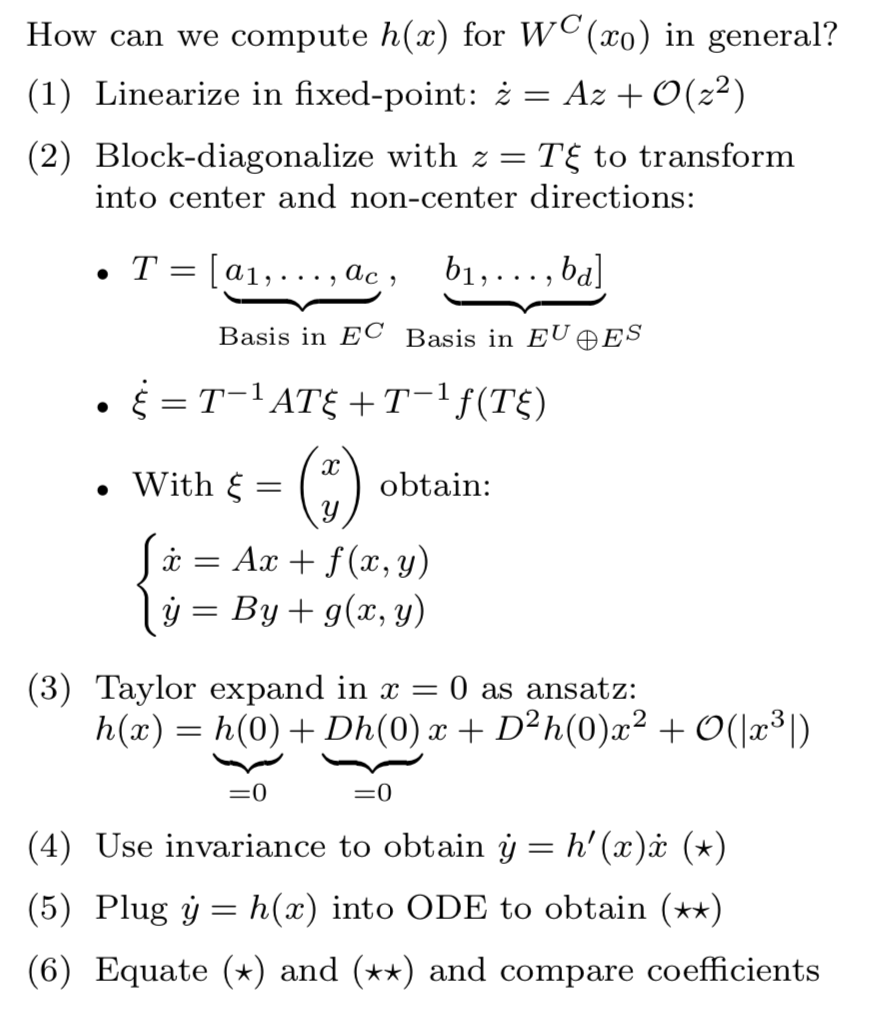
\includegraphics[scale=0.5]{computeWc.png}[h!]


